
\documentclass[10pt]{article}
\usepackage[utf8]{inputenc}
\usepackage{graphicx}
\usepackage{amsmath, amssymb}
\usepackage{geometry}
\usepackage{caption} 
\geometry{a4paper, margin=0.5in, landscape} 

\begin{document}

\section*{Comparative EIS Kinetics Report}
\textbf{Model Structure:} \texttt{R0-p(R1-p(R2,CPE2)-p(R3,L3),CPE1)}

\begin{center}
    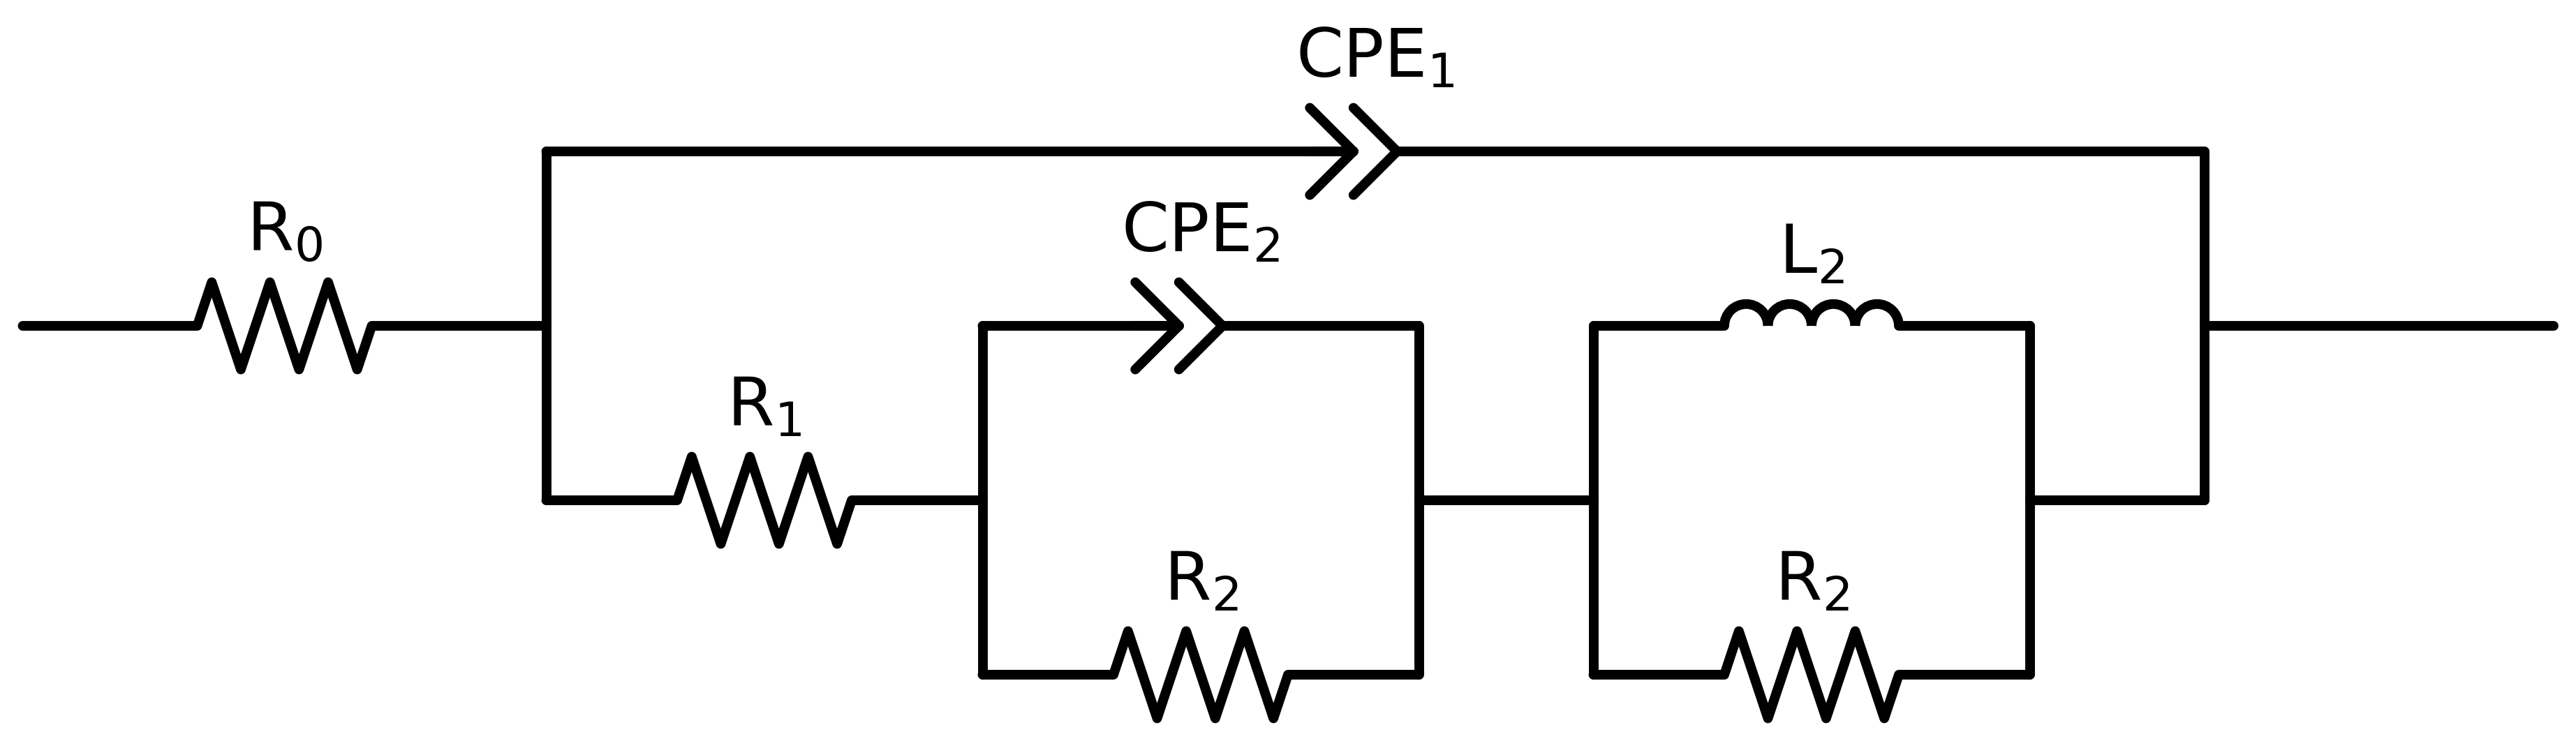
\includegraphics[width=0.45\textwidth]{../../2RC_L.png}
\end{center}

\renewcommand{\arraystretch}{1.6} 
\begin{table}[h!]
    \centering
    \footnotesize
    \begin{tabular}{|l|c|c|c|c|c|}
        \hline
        \textbf{Element} & \textbf{Unit} & \textbf{Bounds} & \textbf{Cauvel\_1\_MBT\_1H} & \textbf{Cauvel\_1\_MBT\_4H} & \textbf{Cauvel\_1\_MBT\_8H} \\ \hline
        $R_{0}$ & $\Omega$ & $[1.0e-03, 1.0e+03]$ & $7.99e+01 \pm 6.6e-01$ & $7.59e+01 \pm 5.0e-01$ & $7.43e+01 \pm 4.5e-01$ \\ \hline
        $R_{1}$ & $\Omega$ & $[1.0e+00, 1.0e+08]$ & $1.50e+05 \pm 1.9e+04$ & $4.41e+05 \pm 5.6e+05$ & $6.75e+05 \pm 2.6e+04$ \\ \hline
        $R_{2}$ & $\Omega$ & $[1.0e+00, 1.0e+08]$ & $1.30e+01 \pm 1.9e+04$ & $1.10e+05 \pm 6.1e+05$ & $2.69e+05 \pm 2.0e+05$ \\ \hline
        $Q_{2}$ & $\Omega$$^{-1}$ sec$^{a}$ & $[1.0e-11, 1.0e-03]$ & $1.10e-10 \pm 3.6e+02$ & $5.75e-06 \pm 7.1e-05$ & $9.36e-05 \pm 7.9e-05$ \\ \hline
        $n_{2}$ & - & $[5.0e-01, 1.0e+00]$ & $6.23e-01 \pm 4.5e-10$ & $5.00e-01 \pm 1.4e+00$ & $1.00e+00 \pm 2.8e-01$ \\ \hline
        $R_{3}$ & $\Omega$ & $[1.0e+00, 1.0e+08]$ & $2.18e+05 \pm 3.2e+04$ & $1.00e+08 \pm 9.8e+00$ & $9.97e+07 \pm 3.7e-01$ \\ \hline
        $L_{3}$ & H & $[1.0e-05, 1.0e+07]$ & $1.75e+06 \pm 6.0e+05$ & $2.28e+04 \pm 2.9e+04$ & $2.58e+04 \pm 3.9e+04$ \\ \hline
        $Q_{1}$ & $\Omega$$^{-1}$ sec$^{a}$ & $[1.0e-11, 1.0e-03]$ & $6.14e-06 \pm 3.1e-07$ & $6.80e-06 \pm 1.0e-07$ & $7.03e-06 \pm 1.0e-07$ \\ \hline
        $n_{1}$ & - & $[5.0e-01, 1.0e+00]$ & $9.26e-01 \pm 6.5e-03$ & $9.12e-01 \pm 2.7e-03$ & $9.06e-01 \pm 2.5e-03$ \\ \hline
        \textbf{$\chi^2$} & - & -  & $1.354e-03$ & $8.708e-04$ & $7.272e-04$ \\ \hline

    \end{tabular}
\end{table}


\newpage
\section*{Analysis Results: 1H}
\begin{center}
    
\includegraphics[width=0.7\textwidth]{plots_Cauvel_1_MBT_1H.pdf}
    \captionof{figure}{EIS Fit Results for Cauvel\_1\_MBT\_1H}
\end{center}

\newpage
\section*{Analysis Results: 4H}
\begin{center}
    
\includegraphics[width=0.7\textwidth]{plots_Cauvel_1_MBT_4H.pdf}
    \captionof{figure}{EIS Fit Results for Cauvel\_1\_MBT\_4H}
\end{center}

\newpage
\section*{Analysis Results: 8H}
\begin{center}
    
\includegraphics[width=0.7\textwidth]{plots_Cauvel_1_MBT_8H.pdf}
    \captionof{figure}{EIS Fit Results for Cauvel\_1\_MBT\_8H}
\end{center}


\end{document}
